

\documentclass[11pt,fleqn]{book} % Default font size and left-justified equations

\input{structure} % Insert the commands.tex file which contains the majority of the structure behind the template
\usepackage{float}

\usepackage{listings} 
\lstset
{ 
    language=C,
    basicstyle=\ttfamily,
    columns=fullflexible,
    keepspaces=true,
    numbers=none,
    stepnumber=1,
    showstringspaces=false,
    tabsize=1,
    breaklines=true,
    breakatwhitespace=false,
    keywordstyle=\color{blue!80!black},
    stringstyle=\color{red!80!black},
    commentstyle=\color{green!40!black},
    morecomment=[l][\color{magenta!80!black}]{\#}
}

\usepackage{caption}
\captionsetup[figure]{font=small,skip=10pt}

%\usepackage{enumitem}
%\setlist{noitemsep} % or \setlist{noitemsep} to leave space around whole list


%%%%% May be too harsh to prevent paragraph breaks across pages! 
%\interlinepenalty 10000
\widowpenalties 1 10000
\raggedbottom


\newcommand{\ilcode}[1]{
    %\vspace{0.5pt}
    \smallskip
    \colorbox{gray!20!white}{
        \centering
        \parbox{\linewidth-2\fboxsep}{
            \lstinline@#1@
        }
    }
    %\vspace{0.5pt}
}

\newcommand{\code}[3]{
    \begin{figure}[]
        \colorbox{gray!20!white}{
            \parbox{\linewidth-2\fboxsep} {
                \centering 
                \lstinputlisting[language=C]{#1}
            }
        }
        \caption{#2}
        \label{#3}
    \end{figure}
}

\usepackage{textcomp}
\usepackage{wrapfig}
\usepackage{float}

\usepackage{silence} % http://ctan.org/pkg/silence
\ErrorFilter{textcomp}{Symbol \textrightarrow not provided}

% Disable paragraph indentation globally since template was indenting some and not others. (looked terrible)
\setlength{\parindent}{0pt}


%%%%%%%%%%%%%%%%%%%%%%%%%%%%%%%%%%%%%%%%%%%%%%%%%%%%%%%%%%%%%%%%%%%%%%%%%%%%%%%%%%%%%%%%%%%%%%%%%
%%%%                                                                                         %%%%
%%%%       Chapter 5: Embedded Communications and the USART                                  %%%%
%%%%                                                                                         %%%%
%%%%%%%%%%%%%%%%%%%%%%%%%%%%%%%%%%%%%%%%%%%%%%%%%%%%%%%%%%%%%%%%%%%%%%%%%%%%%%%%%%%%%%%%%%%%%%%%%

\setcounter{chapter}{4} % Manually adjust chapter counter to number before desired chapter heading

\begin{document}
	
\chapterimage{chapter_head_2.png} % Chapter heading image
\chapter{Embedded Communications and the USART}

\section{Communication Between Systems}
All computing systems regardless of their size and power, are essentially useless if they do not have some way to communicate with the outside world. Even large supercomputers are unable to perform any meaningful work without some method of introducing new data into the systems, and another to output a result. 

Naturally, this applies to embedded systems as well. In fact, the majority of embedded peripherals, as well as these labs, are directed at either capturing or sending information in and out of the system. In the first lab, we introduced the GPIO as the most basic method of data transfer. In the second we used the EXTI controller to allow efficient hardware monitoring of GPIO inputs. The third lab used the capture/compare units in a timer peripheral to generate pseudo-analog signals through PWM. 

This lab introduces the fundamentals of data transfer through digital communication interfaces. These interfaces exist because information is only useful when it can be understood. Therefore there must be defined ways of transmitting and interpreting it.

\subsection{Parallel vs Serial}

There are two main schemes, parallel and serial, for moving binary information across electrical connections. These two schemes are opposites of each other and are demonstrated in figure \ref{parallel_serial}. 

\subsubsection{Parallel}
Parallel interfaces transmit entire blocks of data using multiple wires, with each wire representing the value of a single binary bit. In a parallel system, the transmitter sets the logical state of each wire, and the receiver samples all of the connections at a single instant. Parallel interfaces have a \textit{bit-width} which represents how many wires are in the connection and indicates how many bits are sent at one time. Common bit-widths are powers of 2 to make converting into bytes simple. 

\subsubsection{Serial}
Serial interfaces use a single wire and stream a block of data over time by lining up the bits behind each other. To properly transmit data, both the transmitter and receiver must agree on the time duration between data bits, known as the interface's \textit{bit/data rate}. A serial transmitter produces periodic transitions on the single data line corresponding to the data to be sent. The receiver samples this data line on a similar period and appends the sampled value to the end of the received data. 

\begin{figure}[]
    \centering\includegraphics[width=\textwidth]{parallel_serial}
    \caption{Comparison of parallel and serial communication.}
    \label{parallel_serial}
\end{figure}

\subsubsection{Interface Bandwidth and Limitations}
Because parallel connections move entire groups of bits at a time they have a much higher \textit{bandwidth} (throughput) than an equivalent serial connection. Some examples of high-speed parallel connections are the STM32F0's internal device busses (AHB and APB) which connect the ARM processor core to the SRAM, flash memory and other peripherals.

However, despite that equivalent-speed parallel connections have a higher bandwidth, most high-speed device interfaces such as SATA, USB and Ethernet are serial interconnects. The reason for this is because parallel connections are far harder to design and operate as the distance between the receiver and transmitter increases. With the incredibly high speeds of today's communications, unless every wire in a connection is exactly the same length it is possible to have some bits arrive after the others. This means that unless the sampling rate of the receiver is slow enough to account for every bit of the connection, incorrect data will be captured.

Serial connections inherently don't have issues with wire-delay. Because bits are streamed one after another, any delays along the wire have a consistent effect on the data and can't cause corruption. This enables serial connections to have a much higher bit rate than parallel, and possibly even a higher total bandwidth.

\subsection{Synchronous vs Asynchronous}

Regardless of whether an interface is serial or parallel, there must be a mechanism that synchronizes when the transmitter and receiver updates or samples the connection. Similar to parallel and serial there are two methods, synchronous and asynchronous, of performing this task. These are demonstrated in figure \ref{synchronous_asynchronous}.

\subsubsection{Synchronous} 
Synchronous systems use a separate ``clock'' signal which notifies the receiver when to sample.  Often the data capture is synchronized to a transition such as rising or falling edge. Synchronous systems are often simpler in design but require the extra clock connection.

\subsubsection{Asynchronous}
Asynchronous systems operate without a physical clock signal. Some methods of asynchronous communication encode a virtual clock within the transitions of the data while others estimate the time intervals that data should be expected to arrive. Because of the lack of a clock signal, asynchronous interconnects are typically more complex and have lower data rates than synchronous ones.  

\begin{figure}[]
    \centering\includegraphics[width=\textwidth]{synchronous_asynchronous}
    \caption{Comparison of synchronous and asynchronous serial communication.}
    \label{synchronous_asynchronous}
\end{figure}

\subsection{Connection Topologies} 
The topology of a communication interface is how the different devices (nodes) and the connections between them are arranged. Some interfaces are strictly point-to-point, which means that they connect only two devices with direct wires. Other interfaces have topologies which allow networks of devices to be connected. Figure \ref{topologies} demonstrates a few simple topologies. 

\begin{itemize}
    \item \textbf{Daisy-Chain} -- Nodes in a daisy-chained network connect only to their adjacent neighbors. Some are designed to allow data to be passed along to its destination. 
    \item \textbf{Bus/Multi-Drop} -- All nodes on a bus share the same communication lines. This means that only a single device can be transmitting at a time, but all can receive
    \item \textbf{Star} -- All peripheral nodes communicate with a central master node.
    \item \textbf{Mesh} -- Nodes in a mesh network have arbitrary connections to each other. Some mesh networks are hierarchically ordered, others may be fully-connected.    
\end{itemize}



\begin{figure}[]
    \centering\includegraphics[width=\textwidth]{topologies}
    \caption{Simple network topologies.}
    \label{topologies}
\end{figure}

\section{Communication Standards \& Protocols}

Aside from knowing how to connect and when to sample the inputs, communicating devices must know how to interpret signals into bits and how the patterns of bits make up data. To manage this, all interfaces are combinations of hardware standards and communication protocols. 

\subsection{Hardware Standards}	
Hardware standards define the physical and signaling characteristics of an interface.
A standard typically indicates the medium that the signals are transferred over such as conductive wires, optical, radio frequency or others. The standard defines the method that signals are interpreted into bits. This may be as simple as thresholding a voltage on a wire (single-ended), monitoring the voltage difference or current flow between a pair of wires (differential) or even a modulated waveform. 

Standards often indicate whether an interface is parallel or serial.

\subsection{Communication Protocols}
Hardware standards make it possible to convert an input signal into a collection of bits. However, protocols define the meaning of bits such that they create useful data. 

\subsubsection{Hardware Protocols}
Low level or hardware protocols define how bits are organized to form raw data. This primarily involves the rate that data is sampled and whether the interface has an explicit clock signal or is asynchronous.
Depending on the complexity of the interface, hardware protocols usually include higher-level features such as start/stop signals, error-correction, control flow, message acknowledgment, addressing, data packets and more.

\subsubsection{Software Protocols}	
At this point the communication peripheral's job is complete. Raw data can be converted into a communication signal and back on the receiving end. The last task is to interpret the raw data into useful instructions or information for the user's application.

A software protocol is a device driver that gives meaning to the binary data flowing into and out of the system. These drivers can be as simple as recognizing certain values as commands, or as complex as defining the organization of variable-length data packets.  In order to communicate, the user's application must define a software protocol. 

\subsection{Separating Interface and Protocol}
   
Some communication interfaces have clearly defined separations between the different standards, protocols, and application layers within them. 

For example, IEEE 802.3 is the base standard for wired Ethernet and contains subclasses for the different speeds and modifications that have been made over the years. Built upon these standards are multiple layers of protocols (such as MAC, IP, and TCP) which eventually lead to network sockets that transfer raw data on conventional computer networks. 

An example of a common software protocol used by computer networks is HTML. This format is used to give the browser application a known way to interpret raw text data into a displayed web page. 

Unfortunately, unlike Ethernet, many low-level interfaces such as those used in embedded systems are less clear about where the boundaries are. Many of these interfaces have protocols and standards that were designed specifically for each other and are called by the same name. 
Because of this, many documents use the terms standard and protocol interchangeably. 
 

\section{Common Embedded Interfaces}
The STM32F072 has a generous selection of interface peripherals. These can be seen on the first page summary of the chip datasheet. These interfaces differ widely in operation, complexity, and features; however, they all are serial. 

The three most common serial communication interfaces used in embedded systems are TTL RS-232 (TTL-Serial/UART), Serial Peripheral Interface (SPI), and Inter-Integrated Circuit Bus (I2C). 

This lab teaches the basics of TTL RS-232 in the next few sections. SPI and I2C will be covered in later labs; a brief introduction is included here. 

\begin{itemize}
    \item \textbf{Serial Peripheral Interface (SPI)}
    \begin{itemize}
        \item SPI is a synchronous interface typically used for high-speed connections between microcontrollers and external memories or other fast-data devices.
        \item It is a full-duplex interface, which means that both sides transmit and receive at the same time.
    \end{itemize}
    \item \textbf{Inter-Integrated Circuit Bus (I2C)}
    \begin{itemize}
        \item I2C is a low(er) speed synchronous interface designed to allow multiple master devices to share the same set of signal wires. 
        \item It was primarily intended for low-speed sensors, but newer standards have increased the speed where it is also used for other purposes.
    \end{itemize}
\end{itemize}



\section{Introducing RS-232}
\subsection{Conventional RS-232}
RS-232 was first introduced in 1962 by the Electronic Industries Alliance as a method of connecting teletype terminals to a central computer. It is a point-to-point, asynchronous, full-duplex (simultaneous bi-directional communication) interface with hardware flow control signals. 

Despite changing its voltage levels and connectors over the years, RS-232 became the standard method of interconnection between computers and accessories until it began to be replaced in the late 1980's by PS2 and later USB. Because of its long and common use, RS-232 is often referred to simply as ``Serial.'' 

RS-232 contains features originally designed for slow dial-up connections. The flow control signals allow the transmitter and receiver to directly notify each other that they are ready with new data or that they need a pause to process what has been transmitted. To ensure that the data signal was able to be read across a potentially long cable, RS-232 uses a wide voltage swing with positive voltages representing a `1' and negative voltages for a `0.' Although the standard allows up to {\textpm}25V many devices use between {\textpm}12V and {\textpm}15V.

The most recent and common connector used for RS-232 is the 9-pin trapezoidal DE-9 (often mistakenly called DB-9). Figure \ref{db9_pinout} shows a representation and pinout of the connector. While most consumer equipment does not feature a physical serial port anymore, RS-232 is still commonly used for equipment control within science and industry.  


\begin{figure}[]
    \centering\includegraphics[width=0.3\textwidth]{db9_pinout}
    \caption{Conventional DE9 serial connector and pinout.}
    \label{db9_pinout}
\end{figure} 

\subsection{Embedded TTL RS-232 (TTL-Serial)}
Unlike the original legacy hardware, many embedded systems run at far lower voltages than the  RS-232 {\textpm}25V specification. Additionally, many of these systems cannot generate or tolerate negative voltages. Because of this, most systems use a variant of RS-232 called TTL Serial.

TTL Serial is the same protocol as RS-232 but uses a more reasonable voltage range for signaling. Depending on the power supply that the embedded system operates from, TTL Serial often has a voltage range between 0V and 1.8V to 5V. 

Figure \ref{serial_detail} shows a detailed look into an RS-232 and TTL Serial data frame (packet). As shown, a TTL Serial signal not only has a smaller voltage range, but the waveform is also inverted. 

\begin{figure}[]
    \centering\includegraphics[width=\textwidth]{serial_detail}
    \caption{RS-232 and TTL-Serial logic levels and polarity.}
    \label{serial_detail}
\end{figure}

RS-232 is a very flexible protocol in that many of the communication parameters are adjustable by the user. These next few sections discuss important characteristics of an RS-232 frame.  

\subsubsection{Baud Rate} 
Because RS-232 is asynchronous, both the transmitter and receiver are required to operate on a pre-agreed period between bits. This frequency is known as the \textit{Baud Rate} and represents the number of bits per second that is transmitted. 

RS-232 has no checking mechanism to ensure that both devices are tuned to the same baud. This means that it is possible to receive corrupt data if the baud settings are not configured properly. 

In figure \ref{serial_detail} the bit periods are indicated by alternating white and gray shading. 

\subsubsection{Start and Stop Bits}
Although the official RS-232 protocol does not have a mechanism to detect the receiving Baud rate, it does include \textit{framing bits} which alert the hardware about newly arriving data. 

The first signal transition in figure \ref{serial_detail} is the \textit{start bit} of a data frame. The start bit is used to signal a new data frame and synchronize the clock of the receiver to the transmitter.   

The last transition is the \textit{stop bit} which serves as a spacer to give a minimum delay time before the next frame can start. Originally this was designed to allow the mechanical hardware in the teletype machines to move to the next position in the document.

The number of start and stop bits within a data frame is configurable. Many serial peripherals allow the user to select the number of framing bits. However, similar to the baud rate, both devices need to agree to interpret the data correctly. 
 

\subsubsection{Data Bits} 
Typically each frame in RS-232 contains a single data byte. Although uncommon, the standard allows non-byte data sizes between 5 and 9 bits. The baud rate of the signal includes the framing bits within its calculation of total bits per second. This means that the actual useful data transmitted is always less than the theoretical throughput indicated by the baud. 

\subsubsection{Parity \& Error Checking}
Most hardware peripherals support appending a \textit{parity} bit to the end of the data. Parity is a method of error checking, where the parity bit is set such that the number of `1' bits in each data frame is always even or odd. If the number of received `1' bits fails to match the expected parity, then the hardware can determine that the transmission has been corrupted. 

Parity can only determine if a single bit in the data has been corrupted, it does not provide for any error correction and can fail if an even number of bits are corrupt. Parity is no longer used often because of this limitation. Many devices contain hardware for performing more sophisticated \textit{cyclic redundancy checks} (CRC).  


\subsection{ASCII Text Encoding}

Unlike more sophisticated interfaces, RS-232 does not require any device enumeration or addressing. This enables us to interface with serially connected devices by simply typing characters into a terminal. Regardless of whether a device is attached to the other end is irrelevant, data will be streamed out the transmit line, and any data received will be printed into the terminal console.  

Streaming binary data across a serial link is straightforward. Ideally, the same binary values will be received as was transmitted. However, how is text-based data transfered considering that a serial interface only moves raw bytes? 

Over the years, organizations have created standardized ways to encode text characters as numerical values. One of the oldest of these is the \textit{American Standard Code for Information Interchange} (ASCII). 

ASCII originally assigned a 7-bit value to 128 text characters in the English language. These included upper and lower case letters, numbers, common punctuation marks, and a selection of control codes which modify where and how text was printed in the original teletype machines. Initially, the 8th bit of the byte-wide ASCII encoding was reserved for parity checking. However, this was later changed to allow an additional 128 characters to be added to the extended encoding. 

Only a few of the original control codes still have meaning in modern systems. Examples of these are the `\textbackslash{}t' (Tab) and `\textbackslash{}n' (Newline) characters. Figure \ref{ascii_table} shows some of the more commonly used English characters and their ASCII numerical values.  

In conventional computing, ASCII has largely been replaced by variable-length text encodings such as Unicode. These attempt to include accents and non-Latin characters used by other languages. Although these encodings are far superior to ASCII, they typically keep the old values for the original ASCII characters for backward compatibility. This means that we can successfully use a serial terminal with our embedded systems while only dealing with decoding the original character set.

While it is possible to include a Unicode decoder in an embedded system, the size and complexity may outweigh the potential benefit. Because of this, all text encodings used in the assignments are assumed to be ASCII.

\begin{figure}[]
    \centering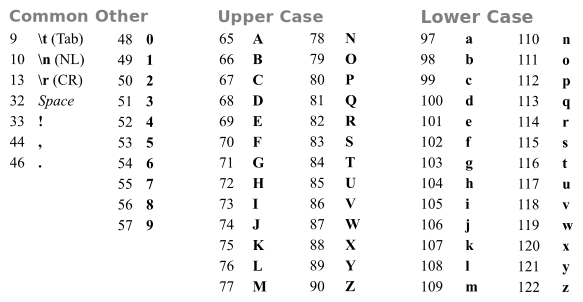
\includegraphics[width=\textwidth]{ascii_table}
    \caption{Subset of the ASCII text encoding standard.}
    \label{ascii_table}
\end{figure}


\section{Introducing the USART}
The \textit{Universal Synchronous Asynchronous Receiver Transmitter} (USART) as suggested by its name, is one of the most flexible communications peripherals available. Its use is common enough that most embedded devices regardless of their manufacturer have multiple USARTs or at the least a simpler Universal Asynchronous Receiver Transmitter (UART).

Although a USART/UART can be configured into a variety of custom communication modes, they are often used to perform basic TTL serial. Sections 27.2 through 27.4 of the peripheral reference manual document the main features of the USARTs found within the STM32F072. From these sections, it is possible to see that the flexibility of the USART makes it appear as a complex device to configure. 

Luckily, due to the popularity of using the USART as a TTL serial device, many of the options that we would normally need to enable are configured by default. The following sections of this lab manual will attempt to provide an overview of each control register used for TTL serial and the options they configure. 

\subsection{USART Registers}	

\subsubsection{Control register 1 (USART\_CR1)}
Control register 1 enables/disables interrupt conditions and portions of the USART peripheral. It sets basic timing and sampling modes as well as the number of data bits in a frame. (The manual calls serial frames ``words''.) 

Note that many bits within the register have a note in their description stating that they are only editable when the USART peripheral has not yet been enabled for communication. 

\subsubsection{Control register 2 (USART\_CR2)}
Control register 2 controls signal polarity and routing for the USART. A common and irritating occurrence when designing circuits is the accidental swap of the receive and transmit lines. Through the control registers, it is possible to swap the signals within the USART peripheral itself. 

Other functions of the control register 2 involve the LIN interface mode and stop bit configuration 

\subsubsection{Baud rate register (USART\_BRR)}
The baud rate register is the prescaler for the USART's baud rate frequency. The value written here can be derived from the processor clock and target communication rate. This will be discussed in the next section of the lab.

\subsubsection{Interrupt and status register (USART\_ISR)}
The interrupt and status register is read-only and indicates different operational states of the USART. Unlike the previously used peripherals, the USART self-clears many of its condition flags once their conditions have been resolved. 

Read the bit descriptions carefully to determine if a flag needs manual attention.

\subsubsection{Interrupt flag clear register (USART\_ICR)}
For the flags that need manual clearing, or if a certain condition needs to be bypassed, the flag clear register allows the user to clear status flags. 

\subsubsection{Receive data register (USART\_RDR)}
The receive data register holds the last completely received byte of data. The USART has an internal buffer which holds in-progress receptions until they have completed successfully. If new data is available and the receive register contains unread data, the USART discards the new information and sets an overrun error condition.

\subsubsection{Transmit data register (USART\_TDR)}
The transmit data register holds the next byte that is waiting to be transmitted. The USART has an internal buffer which holds data currently in the process of transmission. This means that the transmit data register can be safely filled with new data while the previous is still being processed. The USART will signal an empty transmit register with a flag in the status register. 

\subsubsection{Other Control Registers}
These registers contain advanced configuration options primarily for alternate modes of the USART peripheral. While recommended that you browse through them, you will not need to use these for these lab assignments.



\begin{itemize}
    \item \textbf{Control register 3 (USART\_CR3)} -- Manages hardware flow control, DMA, and Smartcard-interface. 
    \item \textbf{Guard time and prescaler register (USART\_GTPR)} -- Used in low-power and Smartcard mode. 
    \item \textbf{Receiver timeout register (USART\_RTOR)} -- Used by Smartcard mode. 
    \item \textbf{Request register (USART\_RQR)} -- Manually triggers USART events/interrupts. 
\end{itemize}

\subsection{Configuring the Baud Rate}	
The baud rate of the USART depends on three factors: the target frequency, the processor clock speed, and the oversampling mode.

Because it is impossible to completely synchronize the clocks between the transmitter and receiver the USART compensates for the inaccuracy by sampling the input much faster than the original baud rate. In the default oversampling mode, the USART samples the input 16-times faster than the bit-rate. It then uses the average of the multiple samples to decide if the bit should be a one or a zero. The USART can reduce the oversampling to 8x to allow more rapid baud rates to be chosen. This mode should only be selected when signal integrity is known to be good.

Section 27.5.4 documents in detail the process of calculating the value to be written in the baud rate register. The simple equation used is as follows:

\begin{equation*}
Baud_{TX/RX} = \frac{f_{CLK}}{USART\_BRR}
\end{equation*}



\begin{example}[Calculating Baud Rate]
    Consider a system with a processor clock prequency of 8 MHz, 16x Oversampling, and a target baud rate of 9600.  
    \begin{align*}
    & Baud\_Divider = 8000000/9600 = 833.33\overline{33} & & USART\_BRR = 833\\[0.25em]
    & Actual\_Baud = 9604 & & Error = 0.05 \%
    \end{align*}
    
\end{example}
    
Most baud rates will not be exactly achievable using the frequencies that the STM32F0's internal oscillator can produce. In general the higher the baud rate in relation to the processor's clock, the greater the error due to clock cycle granularity. When choosing a baud rate, aim for the highest possible standard value that gives reasonable accuracy. Typically, most manufacturers recommend an error of less than 2\%. 


\subsection{Blocking vs Non-blocking Operation}
There are a number of choices to be made when writing code that interfaces with a communication peripheral. Typically you will be sending more data than will fit in a single transmission frame and you will need to wait while the interface alternates between transmitting and requesting more data.

A simple implementation of such a driver could simply poll the condition flags within the USART peripheral until the device becomes ready to continue. This style of driver is called \textit{blocking,} because it stops the progression of the application thread until the transmission has completed. Depending on the timing of the main application, this may not be a problem. However, a blocking driver cannot be used in an interrupt because of the delays it causes. 

\textit{Non-blocking} drivers use interrupts and buffers to store and move data into the peripheral. A non-blocking driver executes rapidly because the data to transmit is only moved into a storage butter. When there is data within the storage buffer, an interrupt is enabled which triggers whenever the transmit register within the USART becomes available. 

The exercises in this lab will mostly use blocking-style drivers. Although non-blocking drivers for USARTs are simpler than those for most other interfaces, designing one is outside the time scope of a single lab. 
%\figure \ref{blocking_nonblocking} demonstrates
%
%\begin{figure}[]
%    \centering\includegraphics[width=\textwidth]{blocking_nonblocking}
%    \caption{Blocking and non-blocking drivers.}
%    \label{blocking_nonblocking}
%\end{figure}
%\subsubsection{Performing Basic Transmits and Receives}
%
%Figure \ref{blocking_flowchart} shows a flowchart for simple blocking USART drivers on the STM32F0. These flowcharts will be useful on your lab assignments. 
%
%After peripheral initialization, the basic operation of a blocking USART driver follows these basic steps:
%\begin{enumerate}
%    \item Application code produces or requests data.
%    \item Poll until a status bit indicates that the peripheral is ready for the action.
%    \item Move or load the data into or from the appropriate register.
%    \item If more data is waiting to be processed, return to step 2.
%    \item Continue with the original application.
%\end{enumerate}


%\begin{figure}[]
%    \centering\includegraphics[width=\textwidth]{blocking_flowchart}
%    \caption{Flowchart for simple RX/TX communications on the USART.}
%    \label{blocking_flowchart}
%\end{figure}
%Explicitly say when they need to wait/check a flag for this condition before moving onward. 
%Don't give actual bit names, but they should be able to use the register descriptions to know where to look
%Give pretty obvious hints as to what they should look for when searching for bits.
\subsubsection{Text Formatting}
This lab requires a few functions that perform basic string operations. To implement these, you will need to how the c-language represents and terminates character strings. 

The c-standard libraries, which provide conventional string operations, are not available for the STM32F0. These expect a more traditional environment with a freely available heap and plenty of stack and code space. However, there are a few versions of the standard libraries intended for embedded system use. Kiel provides a miniature version of the c-standard library called \textit{microlib} within the ARM:MDK toolchain.

If configured properly it becomes possible to use standard printing functions such as \texttt{printf()} with the USART. This may be discussed in later labs. 


\section{Using a USB-UART Cable and the Terminal}
\subsection{The USB-UART Cable}
Because it is unlikely that consumer computers have native TTL Serial interfaces, many chip vendors sell devices that act as a protocol bridge between USB and TTL Serial. These are built into cables or small circuit boards and often called USB-Serial or USB-UART converters. 

Although these devices are almost universal, this lab suggests using the Adafruit 954 USB-UART cable. This cable directly connects to the USB port of a desktop computer and outputs 3.3V TTL Serial on a 4-pin wire connector. 

Figure \ref{usb_uart} shows an image of the Adafruit 954 cable along with a pinout of the wire headers. To connect the USB-UART cable to the discovery board, first, attach the black GND wire on the cable to one of the matching pins on the board. 

Both the USB-UART cable and the USART on the STM32F0 have receive (RX) and transmit (TX) lines. To communicate, the transmitter of one device must be connected to the receiver of the other. If necessary, refer to the following when connecting the cable to the board. \\

\parbox{\textwidth} {
    \centering
    \textbf{USB-UART Transmit (TX) \textrightarrow  STM32F0 Receive (RX) \\
    USB-UART Receive (RX) \textrightarrow  STM32F0 Transmit (TX)}
}
    

\begin{warning}
When connecting the USB-UART cable to the Discovery board, do \textbf{not} attach the 5V output while debugging. 

This is because the ST-Link already provides 5V power and unless the two sources have equal voltages, current will flow through the supplies, possibly causing damage. 

If both cables are sourced from the same computer, then it is unlikely that there will be issues. However, the extra connection is unnecessary.
\end{warning}

\begin{figure}[]
    \centering\includegraphics[width=0.6\textwidth]{usb_uart}
    \caption{Pinout of the Adafruit 954 USB-UART cable.}
    \label{usb_uart}
\end{figure}

\subsection{Finding Installed Ports on Windows}
When connected to a desktop or laptop computer, USB-UART cables usually appear as virtual RS-232 serial ports to the operating system. Although most adapters work with all common operating systems, because the Kiel toolchain operates on Windows, this lab does not document the steps to find the virtual port on others. 

Whenever new hardware is installed on Windows, the operating system assigns a device name indicating its type and a unique identifier. Serial ports (virtual or physical) are assigned names beginning with ``COM'' and ending with a number. For example, the third serial port installed on a Windows system would be named ``COM3.''

Unfortunately, it is not always easy to determine what name the computer has assigned to the connected cable. Windows creates a new device ID for each unique cable that is connected and has an odd habit of occasionally creating new identifiers for known ones. 

The most reliable method of determining what name has been given to a connected USB-UART cable is to check the Windows, device manager. Figure \ref{device_manager} shows the device manager with a connected cable and the assigned name circled. 

The following steps can be used to open the device manager.

\begin{enumerate}
    \item \textbf{Open the Windows Control Panel} -- The control panel can be accessed from the start menu or all applications view of the home screen.
        \begin{itemize}
            \item If using Windows 8/10 you will need to access the original control panel not the simplified settings app.
        \end{itemize} 
    \item \textbf{Select the Appropriate Category}
     \begin{itemize}
        \item Windows 8/10 -- Select \textit{Devices and Printers} Category
        \item Windows 7 -- Select \textit{System} Category
    \end{itemize} 
    \item \textbf{Select the Device Manager} -- The device manager should be located within the selected category.
\end{enumerate}

Once opening the device manager, expand the \textit{Ports (COM \& LPT)} category. If the category is not visible then Windows has not recognized the device, the drivers may not have automatically installed. In this event visit the product page on Adafruit.com and manually install the cable driver.  
\begin{figure}[]
    \centering\includegraphics[height=0.45\textheight]{device_manager}
    \caption{Windows device manager with the ports tab expanded.}
    \label{device_manager}
\end{figure}

\subsection{Using the Putty Terminal Program}

%\begin{figure}
%    \centering\includegraphics[height=0.15\textwidth]{putty_icon}
%    \caption{Putty terminal icon}
%\end{figure}

\begin{wrapfigure}[8]{h!R}{0.2\textwidth}
    \centering\includegraphics[height=0.15\textwidth]{putty_icon}
    \caption{Putty terminal icon}
    \label{uvision_logo}
\end{wrapfigure}

Putty is a multi-protocol terminal primarily used for accessing remote secure-shell (SSH) connections on Unix/Linux based operating systems. However, it among with many other terminal applications can be used for serial communication.

After launching Putty, the main settings window should open as shown in figure \ref{putty}. There are three steps to configure Putty into the proper mode to communicate with the Discovery board. 
\begin{enumerate}
    \item Select the serial mode using the \textit{Connection Type} option. 
    \item Type the port name for the USB-UART cable in the \textit{Serial Line} box.
    \item Select a baud rate to communicate at in the \textit{Speed} box.
\end{enumerate}

After configuring Putty, click the \textit{open} button. If an error appears, it is likely you have selected a serial name that doesn't currently exist. In this event open the device manager and check for the connected cable's ID. 

If there aren't any errors, a blank terminal window should open. If you type text in the terminal, you should not see any text appearing. This is because the default behavior of the terminal is only to display data that is received from the remove device. (Discovery Board) 

Connecting the transmit and receive lines of the USB-UART cable together using a jumper wire forms a loopback interface. A loopback interface sends data on the transmit and receives it immediately back because the input and outputs are directly connected. In this event, you will see the typed text in the terminal. 

\begin{figure}[]
    \centering\includegraphics[height=0.40\textheight]{putty}
    \caption{Putty terminal settings screen}
    \label{putty}
\end{figure}



\section{Lab Assignment}
Within this lab's exercises you will be connecting the Discovery board to a PC through a USB-UART cable. The first few are designed to familiarize you with the basic concepts of transmitting and receiving data using blocking methods. The final exercise implements a simple character-based command parser which you can use to modify the LEDs on the board.  

\subsection{Preparing to use the USART} 
Unlike the previous labs these exercises involve multiple devices. This makes debugging slightly more complicated because there are now possible connection and software errors due to the cable and PC. Before writing the embedded application, you may want to perform a loopback test by connecting the transmit and receive lines on the adapter cable to ensure that the serial terminal is communicating with the correct virtual port. 

The STM32F072 has four USART peripherals available; you will need to select one of these to use. Each USART has a small selection of GPIO pins that can be used as its transmit (TX) and receive (RX) signals. Because the split connections on the end of the Adafruit USB-USART cable are fairly short, you will want to choose USART output/input pins that are relatively near a GND pin.
 
 \begin{enumerate}
     \item Using the chip datasheet, locate pins that connect to TX/RX signals on USART peripherals.
     \item Choose a set of RX/TX pins that are near enough to a GND connection such that the USB-USART cable's wire ends can reach. 
     \item Connect the USB-UART transmit (TX) line to the STM32F0's receive (RX) pin. Likewise, connect the  STM32F0's transmit (TX) pin to the USB-UART receive (RX) line.
     \item Set the selected pins into alternate function mode and program the correct alternate function number into the GPIO AFR registers. 
     \item Note the USART that the selected pins connect to, this is the peripheral you will be using in the lab exercises.  
 \end{enumerate}

\begin{warning}
    Ensure that both the Discovery board and USB-UART cable areunpowered when connecting them to each other. If one device is connected to the PC and the other is not, the transmit line on the powered device will feed voltage into the unpowered device through its input pin. 
\end{warning}

\subsection{Blocking Transmission}	
This exercise transmits single characters to the serial terminal on the PC. The character transmission will be handled in the main loop of the application using a blocking method. 

\subsubsection{Initializing the USART}
The lab manual mentions all of the registers that you may be required to modify throughout these exercises. Because TTL Serial is the default mode of the USART, many of the configuration bits will already be at their desired state. 

\begin{enumerate}
    \item Enable the system clock to the desired USART in the RCC peripheral.
    \item Set the Baud rate for communication to be 115200 bits/second. 
    \begin{itemize}
        \item You may use the \texttt{HAL\_RCC\_GetHCLKFreq()} function to get the system clock frequency. 
    \end{itemize}
    \item The USART starts with portions of the peripheral disabled for low-power use. You will need to enable the transmitter and receiver hardware.
    \item The USART has a peripheral enable/disable bit in its control register. Once the USART is enabled, many of the configuration bits become read-only.  
\end{enumerate}

\subsubsection{Transmitting a Character}

Write a function that transmits a single character on the USART. Start with a function declaration that accepts a single character-type variable and returns nothing. Within this function implement the following.

\begin{enumerate}
    \item Check and wait on the USART status flag that indicates the transmit register is empty.
    \begin{itemize}
        \item You can use an empty \texttt{while} loop which exits once the flag is set. 
        \item Don't use the USART ``BUSY'' status bit. Although this will appear to work properly, this bit depends on multiple conditions and will slow down your transmission. 
    \end{itemize}
    \item Write the character into the transmit data register. 
    \begin{itemize}
        \item Remember that c-language characters are really numerical values. (ASCII) You can modify and write them to registers without special syntax or type casting.  
    \end{itemize}
    \item There is no need to manually clear the status bit, it will be automatically modified by the peripheral when you write into the transmit register.
\end{enumerate}

Implement some code in the infinite \texttt{while} loop of the main function that calls the character transmit function with a character constant. Feel free to simply loop with delay, or use the button to trigger the transmit. Remember that C-language character constants are surrounded by single quote marks.

\subsubsection{Transmitting a String}
Unlike many other languages, C has no built-in string data type. Instead, text strings are built from arrays of characters. Because C arrays don't have any method of determining how long they are, string constants that are converted by the compiler into arrays are terminated with a null character. The null character `{\textbackslash}0' has the literal ASCII value of 0 and is used as a sentinel (guard) value to let string processing functions know they've reached the end of the array. 

To transmit strings, begin with a function declaration that accepts an array of characters, either in direct array form or as a pointer. This function should loop over each character in the array and call your character transmit function. 

\begin{enumerate}
    \item Loop over each element in the character array
    \item If the current element is not the null character use your character transmit function.
    \begin{itemize}
        \item You can increment over the array by using a counter and array index or by incrementing the pointer.
        \item You can test for the null character by comparing the value against `{\textbackslash}0' or the numerical value 0. (remember characters are numbers in C) 
        \item If you use the pointer method, remember to dereference when testing for the null value and when calling the character transmit function.
    \end{itemize} 
    \item Return when the null character is encountered. 
\end{enumerate}

Once your string transmit function is complete, change your main application to transmit a short phrase instead of a single character. If you see large amounts of garbage printed in the terminal instead of your phrase, you probably have run off the end of your character array and are displaying the contents of the rest of the STM32F0's memory. 

\subsection{Using a Protocol Analyzer}
The true benefit of using logic analyzers is when debugging communications between multiple devices. Connect one of the inputs of a logic analyzer to the transmit pin of the USART. You can do this by using the other side of the pin as the USB-UART cable on the Discovery board.

Once connected, set the trigger for falling-edge and capture a section of the transmission. Using the online user guide linked in the lab Canvas page, apply the \textit{Async Serial} protocol analyzer to the captured trace. 

When configuring the protocol analyzer you should be able to leave all of the settings except the baud rate as default. Once the analyzer has been applied, zoom onto the captured trace until you can see the decoded values above the signal transitions. \textbf{Save a screenshot of the decoded signal for your postlab. }

If the analyzer indicates multiple framing errors, you may have the incorrect baud selected. Click the small gear button on the analyzer tab and change the settings to use Autobaud. Hopefully this will detect the baud rate of your signal and decode properly. 



\subsection{Blocking Reception}

For this exercise you will use the infinite \texttt{while} loop in the main function to read single-character commands typed at the serial terminal on the PC. Your goal is to develop an application that toggles the correct LED whenever the character matching the first letter of the color is pressed. For example, typing an `r' into the terminal would toggle the red LED. 

\begin{enumerate}
    \item Check and wait on the USART status flag that indicates the receive (read) register is not empty.
    \begin{itemize}
        \item You can use an empty \texttt{while} loop which exits once the flag is set or simply check each iteration of the main infinite loop. 
        \item It may be helpful to carefully read the bit descriptions in the register map.
    \end{itemize}
    \item Test the received data and toggle the appropriate LED
    \begin{itemize}
        \item The receive register can be read like an ordinary variable. However, the data isn't guaranteed to remain in the register after it has been read once. 
        \item Unless you use a switch statement you may want to save the value into a local variable and test against that. 
    \end{itemize}
    \item Whenever a key is pressed that doesn't match an LED color, print an error message to the console. 
    \item You will probably want to comment or remove any old transmit code and delay statements from the infinite loop. 
    \begin{itemize}
        \item The possible reception rate at 115200 Baud is faster than the minimum delay the HAL library functions are designed to provide. 
        \item It is possible to lose received data while waiting for a blocking transmit to complete. Where we are only receiving single bytes it is unlikely to cause problems.
    \end{itemize}
\end{enumerate}


\subsection{Interrupt-Based Reception}
In this final exercise you will use an interrupt to save the received data when it arrives. Additionally you will expand your simple command parser with more complex behavior.

\begin{enumerate}
    \item In the USART initialization, enable the receive register not empty interrupt.
    \item Enable and set the USART interrupt priority in the NVIC.
    \item Setup the blank interrupt handler.
    \item Within the handler, save the receive register's value into a global variable.
    \item Within the handler set a global variable as a flag indicating new data. 
\end{enumerate} 

Examine the status flag documentation for the receive register not empty interrupt. You should notice that the USART peripheral automatically clears the flag whenever the receive data register is read. Because of this there is no need to manually clear the bit within the interrupt handler. \\

In this exercise we are saving the contents of the receive register to a global variable. Technically since we are only operating on a single byte, using the interrupt doesn't offer us much of a benefit. This is because saving the data to a simple variable doesn't protect us from losing data if the main loop takes too long and the USART overwrites it with a new value. In better non-blocking implementations a buffer is used; possibly raising the new data flag only after a certain character such as a newline is received.\\

Now that the interrupt is ready, you will need to rewrite your main application to check and act on the flag and data variables you set in the interrupt handler. This portion is an open-ended exercise, you are free to implement it in any method you choose as long as the following requirements are fulfilled. 



\begin{enumerate}
    \item Your command parser must now accept two character commands.
    \begin{itemize}
        \item The first character is a letter matching the one of the LED colors.
        \item The second character is a number between 0 and 2. 
        \begin{itemize}
            \item `0' turns off the LED
            \item `1' turns on the LED
            \item `2' toggles the LED
        \end{itemize}
    \end{itemize}
    \item Print a command prompt such as ``CMD?'' when waiting for user input.
    \item Entering an unknown character prints an error message and restarts back to the beginning.
    \item On a successful command, print a message about which command was recognized. 
\end{enumerate}




%Receive single chars in loop from terminal
%toggle LEDs on char match (r for red etc...)
%\subsection{Interrupt-Based Reception and Command Parsing}	
%Set up USART RX interrupt
%set up static buffer (with basic over/underflow protection)
%buffer word until newline and set flag
%Use simple state machine and string match (they can write) in main program to recognize simple command strings (example: "red \\n on \\n")
%Provide text feedback "ready for command", "buffer overflow", "unknown command", "invalid command", "command accepted"
%\begin{figure}[]
%    \centering\includegraphics[width=\textwidth]{command_flowchart}
%    \caption{Flowchart for command parsing.}
%    \label{command_flowchart}
%\end{figure}


\end{document}
